\documentclass[a4paper,12pt]{article}


\usepackage{minted}
\usepackage[cm]{fullpage}
%\usepackage[a4paper,margin=1in]{geometry}
\usepackage{graphicx}
\usepackage{amsmath}
\usepackage{capt-of}

\setminted[C]{fontsize=\small, tabsize=4, breaklines, linenos}
\setminted[Ruby]{fontsize=\small, tabsize=4, breaklines, linenos}
\setminted[text]{fontsize=\small, tabsize=4, breaklines, linenos}

%\setlength\parindent{0pt}

\title{Assignment 1 Report}
\author{Julius Putra Tanu Setiaji (A0149787E), Chen Shaowei (A0110560Y)}
\date{1 October 2018}

\begin{document}
	\maketitle
	
	\section{Program Design}
	This train simulation is implemented in OpenMP. Primary design considerations are:
	\begin{itemize}
		\item Each train is simulated by one thread as required in the specifications.
		\item This is achieved by calling \mintinline{C}{omp_set_num_threads(num_trains);}
		\item Each train stores its next state, and when it will enter that state.
		\item Each train will generate the time at which it will open its doors when it starts waiting at a station.
	\end{itemize}
	
	\subsection*{Assumptions}
	
	\begin{itemize}
		\item Only one train can open its doors at each at any one time, regardless of direction.
		\item Train stations have infinite capacity for waiting trains.
		\item Time units are discrete and can have no subdivisions
		\begin{itemize}
			\item \textbf{Implication}: It is sufficient to store all time units as integers instead of floating point numbers
		\end{itemize}
		\item Trains must open their doors for at least 1 unit of time.
		\begin{itemize}
			\item \textbf{Implication}: We round every randomly generated door open time up to the nearest integer
  		\end{itemize}
	\end{itemize}
	
	\section{Points to Note / Implementation Details}
	\begin{itemize}
		\item Current simulation time needs to be shared across all threads. In addition, time can only be advanced after all threads have completed the actions to be done in the current tick.
		\item Each train is a finite state machine with 4 states: \texttt{OPEN\_DOOR}, \texttt{CLOSE\_DOOR}, \texttt{DEPART} and \texttt{ARRIVE}.
		\item Each train keeps track of its next action time (time for it to change to the next state), and actions to be completed within the current tick are performed in a \mintinline{C}{while} loop.
		\item There is a \mintinline{C}{#pragma omp barrier} to ensure that all threads exit the \mintinline{C}{while} loop before time is advanced.
		\item The advancement of time is done in a \mintinline{C}{#pragma omp single} block to ensure that it is only performed by one thread. In addition, \mintinline{C}{#pragma omp single} has an implicit barrier at the end of the block so this prevents other threads from entering the next iteration of the \mintinline{C}{while} loop until the advancement of time is complete.
		\item Certain resources i.e. train tracks, door-opening rights are limited, and only one train may access them at any time.
		\begin{enumerate}
			\item One way to implement this is to have threads block when waiting to access such resources. However, this would interfere with the way we have chosen to implement time within this simulation. Blocked threads would prevent code after a \mintinline{C}{#pragma omp barrier} statement from being executed. We therefore decided \textbf{not} to go with this implementation.
			\item An alternative way to implement is to have a queue of trains requesting access to such resources. At each tick, each train would check whether it is at the head of the queue, and if so, it will be able to access the resource. We realised that it will also be necessary to store the time at which a train would be able to gain access to the resource, since our simulation time advances in integer increments, but door open time may have a fractional value. Upon further consideration, we realised that this design could be simplified.
			\item The key insight we arrived at is that any train waiting for access to a resource only needs to know the next time said resource will be available. Since this system does not permit a train to give up waiting for a resource, this can be implemented simply with a thread-safe timekeeper object. When a train requests access to a resource, it tells the timekeeper how much time it will occupy the resource for. The timekeeper will then inform the tra in of the time when the train can access the resource, and update its internal next available time. This is the implementation we decided to go with. In another word, we are implementing an implicit queue for a First-Come-First-Serve (FCFS) scheduling.
		\end{enumerate}
		\item The next consideration is ensuring that system statistics are reported correctly. Since we assume that trains cannot open its doors for 0s, only one train can open its doors at each station per tick. There is therefore no potential race condition in the update of statistics.
		\item Since print statements are not atomic, we wrapped them in a \mintinline{C}{#pragma omp critical} block to ensure that only one print operation executes at any one time.
	\end{itemize}
	
	\section{Execution Time}
	
	\subsection{Testcase Used}
	We use a map generated by a Ruby script which can be found in appendix. The map generated will have at least 4 vertices with degree = 1, and all the paths forming the train lines are at least of length 4. However, these values are configurable.
	
	We ran the same map for 100, 1000, and 10000 time-ticks with all possible different combinations of numbers of trains in each line as long as the total number of trains is between 1 and 64 inclusive. This results in around 47,900 testcases for each time-tick size. As such, we will only include the scatter diagram of the results in the report. However, should the need arise, csv files containing the raw data is attached together with the report.
	
	Below you can find a sample input and visualisation of the adjacency matrix and the train lines. The parameters that we used are number of stations = 10, maximum distance between stations = 10.
	
	Do also note that to facilitate more accurate execution time analysis, we disabled per-tick status output for the following tests.
	
	\begin{center}
		\captionof{figure}{Sample Input}
		\begin{minted}{text}
10
Somerset,Tan Kah Kee,Redhill,Sembawang,Riviera,Samudera,Sengkang,Boon Lay,Tampines West,Tampines
0 0 0 0 0 0 0 0 6 0
0 0 1 0 0 0 1 0 4 1
0 1 0 0 6 0 0 0 0 0
0 0 0 0 0 0 0 4 0 9
0 0 6 0 0 0 0 0 0 0
0 0 0 0 0 0 0 0 0 10
0 1 0 0 0 0 0 0 0 0
0 0 0 4 0 0 0 0 0 0
6 4 0 0 0 0 0 0 0 0
0 1 0 9 0 10 0 0 0 0
0.1,0.2,0.1,0.1,1.0,0.5,0.7,0.8,0.5,0.5
Somerset,Tampines West,Tan Kah Kee,Tampines,Sembawang,Boon Lay
Samudera,Tampines,Tan Kah Kee,Sengkang
Somerset,Tampines West,Tan Kah Kee,Sengkang
10000
21,22,21
		\end{minted}
	\end{center}
	
	\begin{center}
		\captionof{figure}{Map of the train line used, with the 3 lines indicated}
		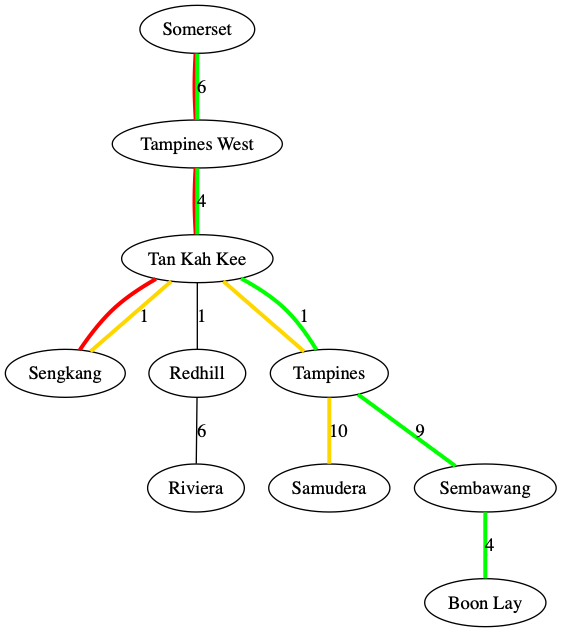
\includegraphics[width=0.5\linewidth]{map}
	\end{center}

	\newpage
	\subsection{Graphs}
	Extreme outliers were removed from the scatter diagram.
	\begin{center}
		\captionof{figure}{Execution Time for 100 ticks}
		\centering
		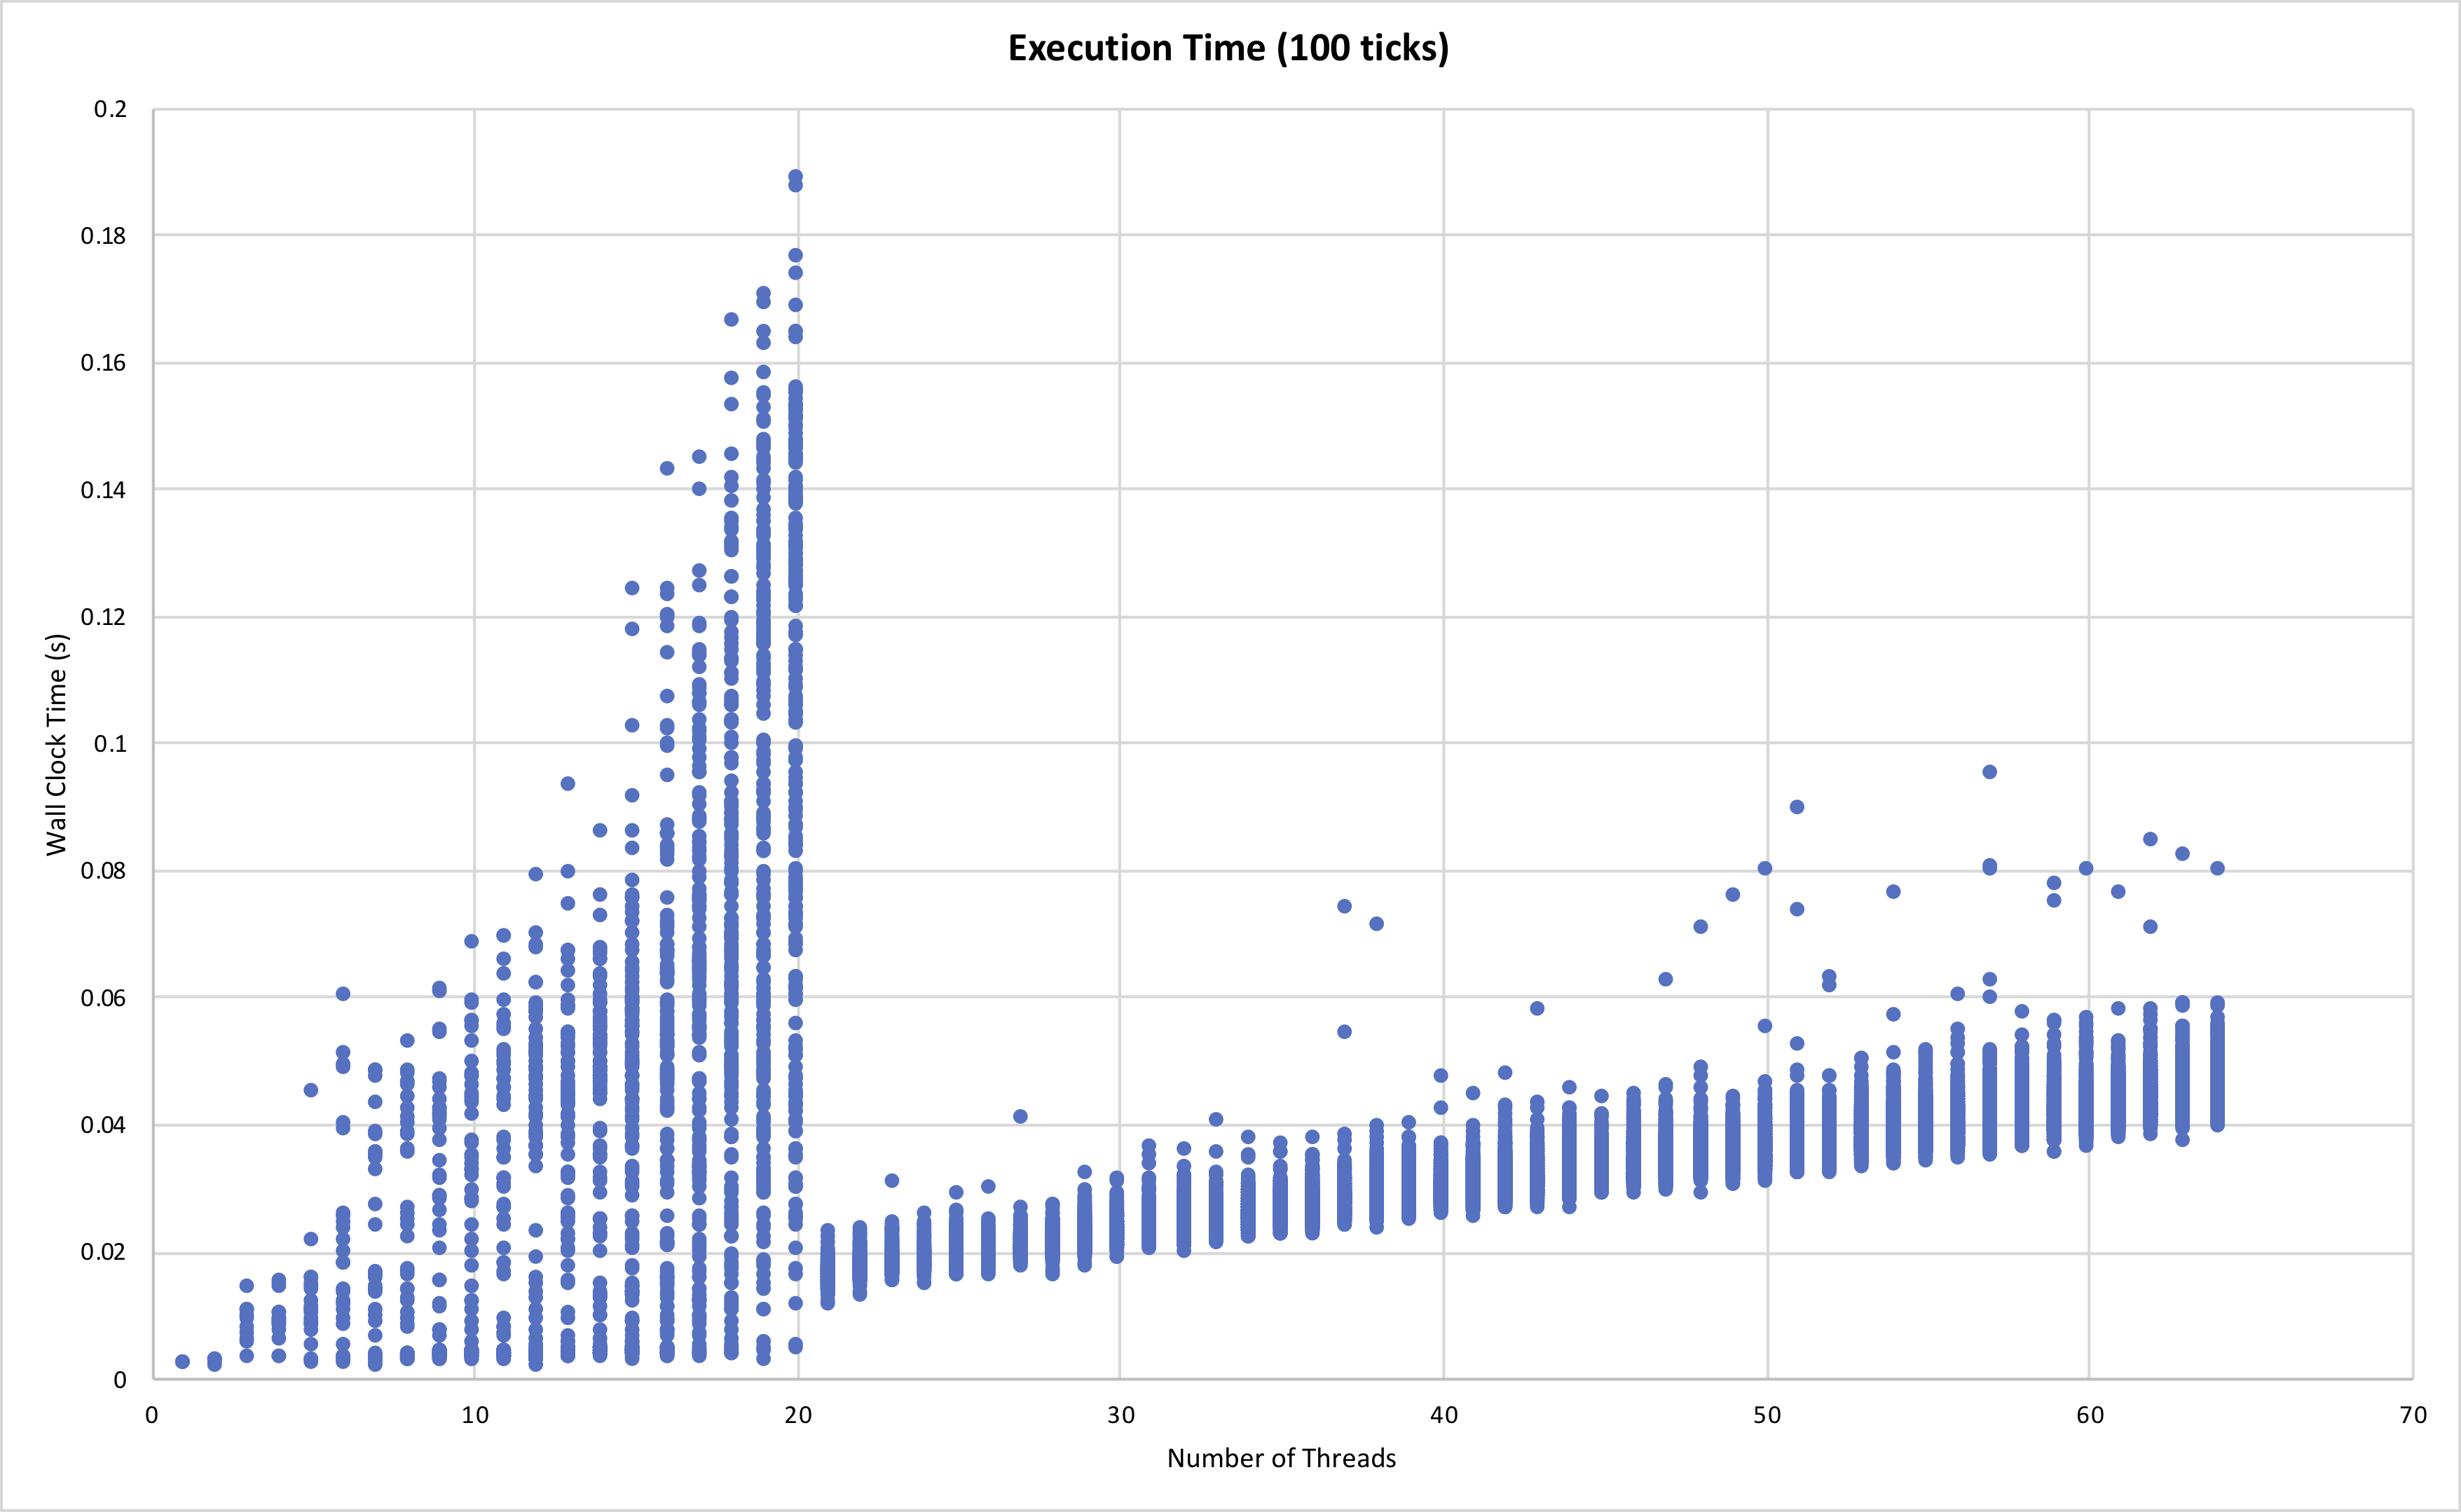
\includegraphics[width=\linewidth]{100-time}
	\end{center}
	\begin{center}
		\captionof{figure}{Execution Time for 1,000 ticks}
		\centering
		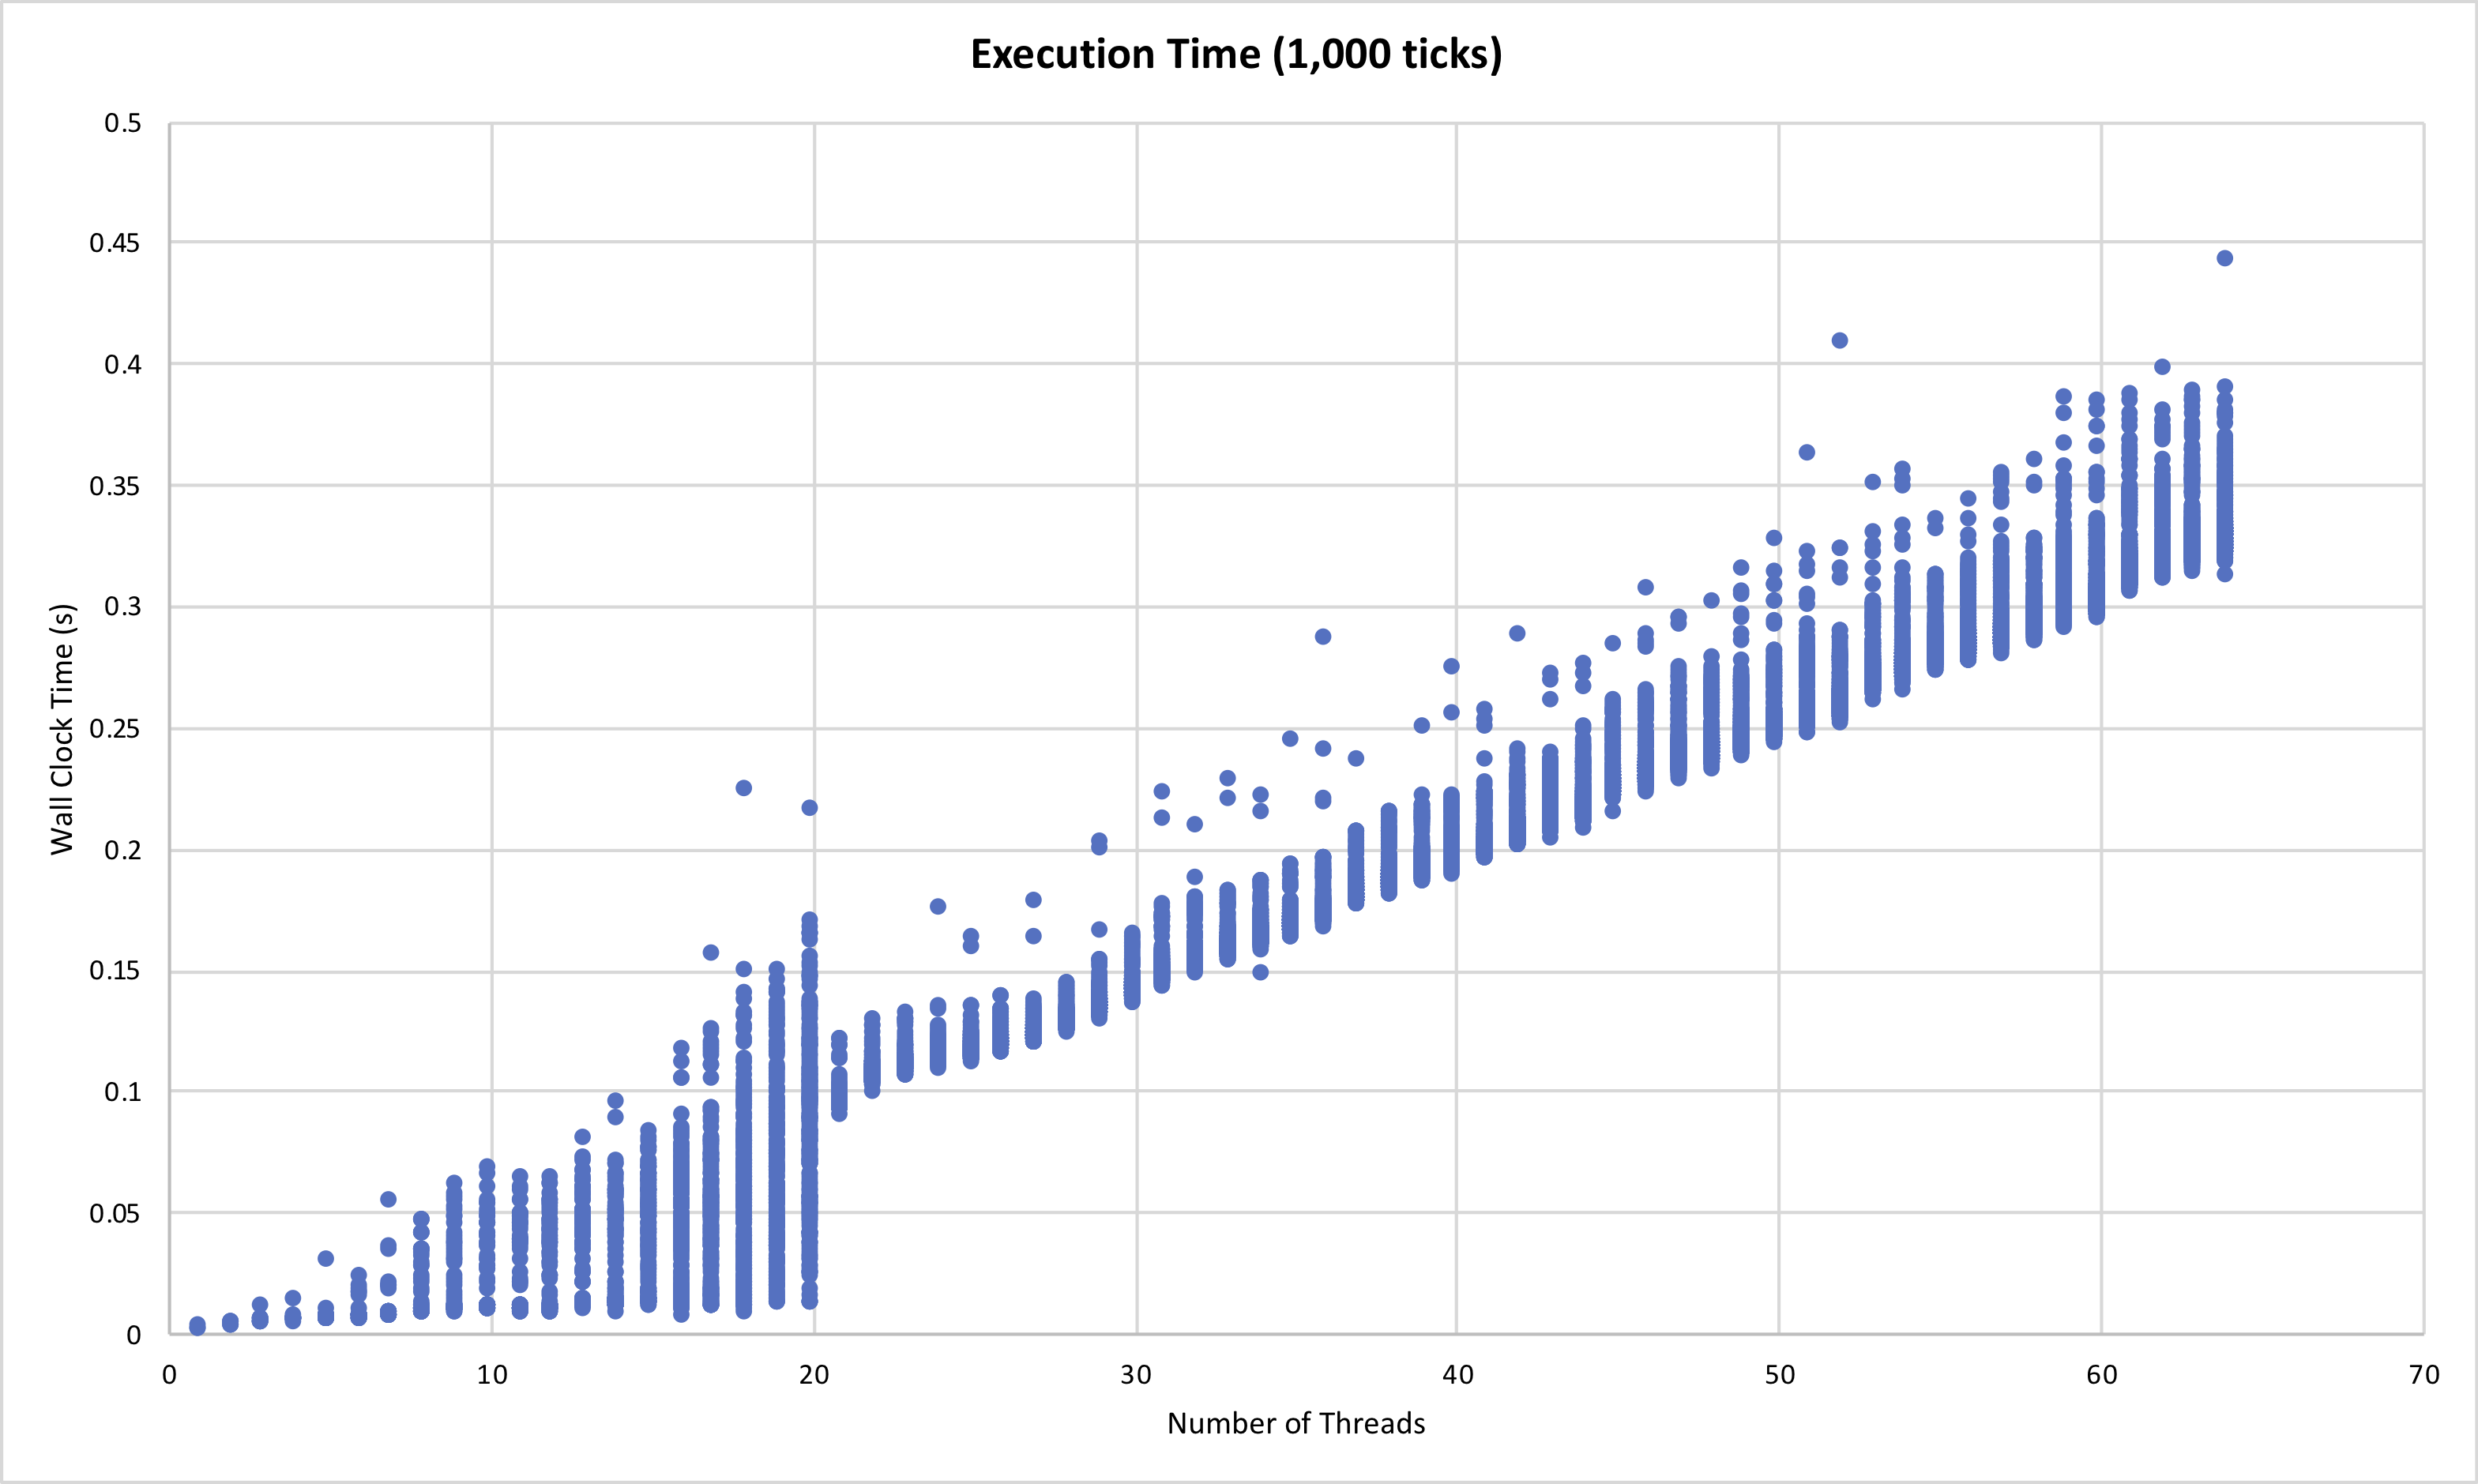
\includegraphics[width=\linewidth]{1000-time}
	\end{center}
	\begin{center}
		\captionof{figure}{Execution Time for 10,000 ticks}
		\centering
		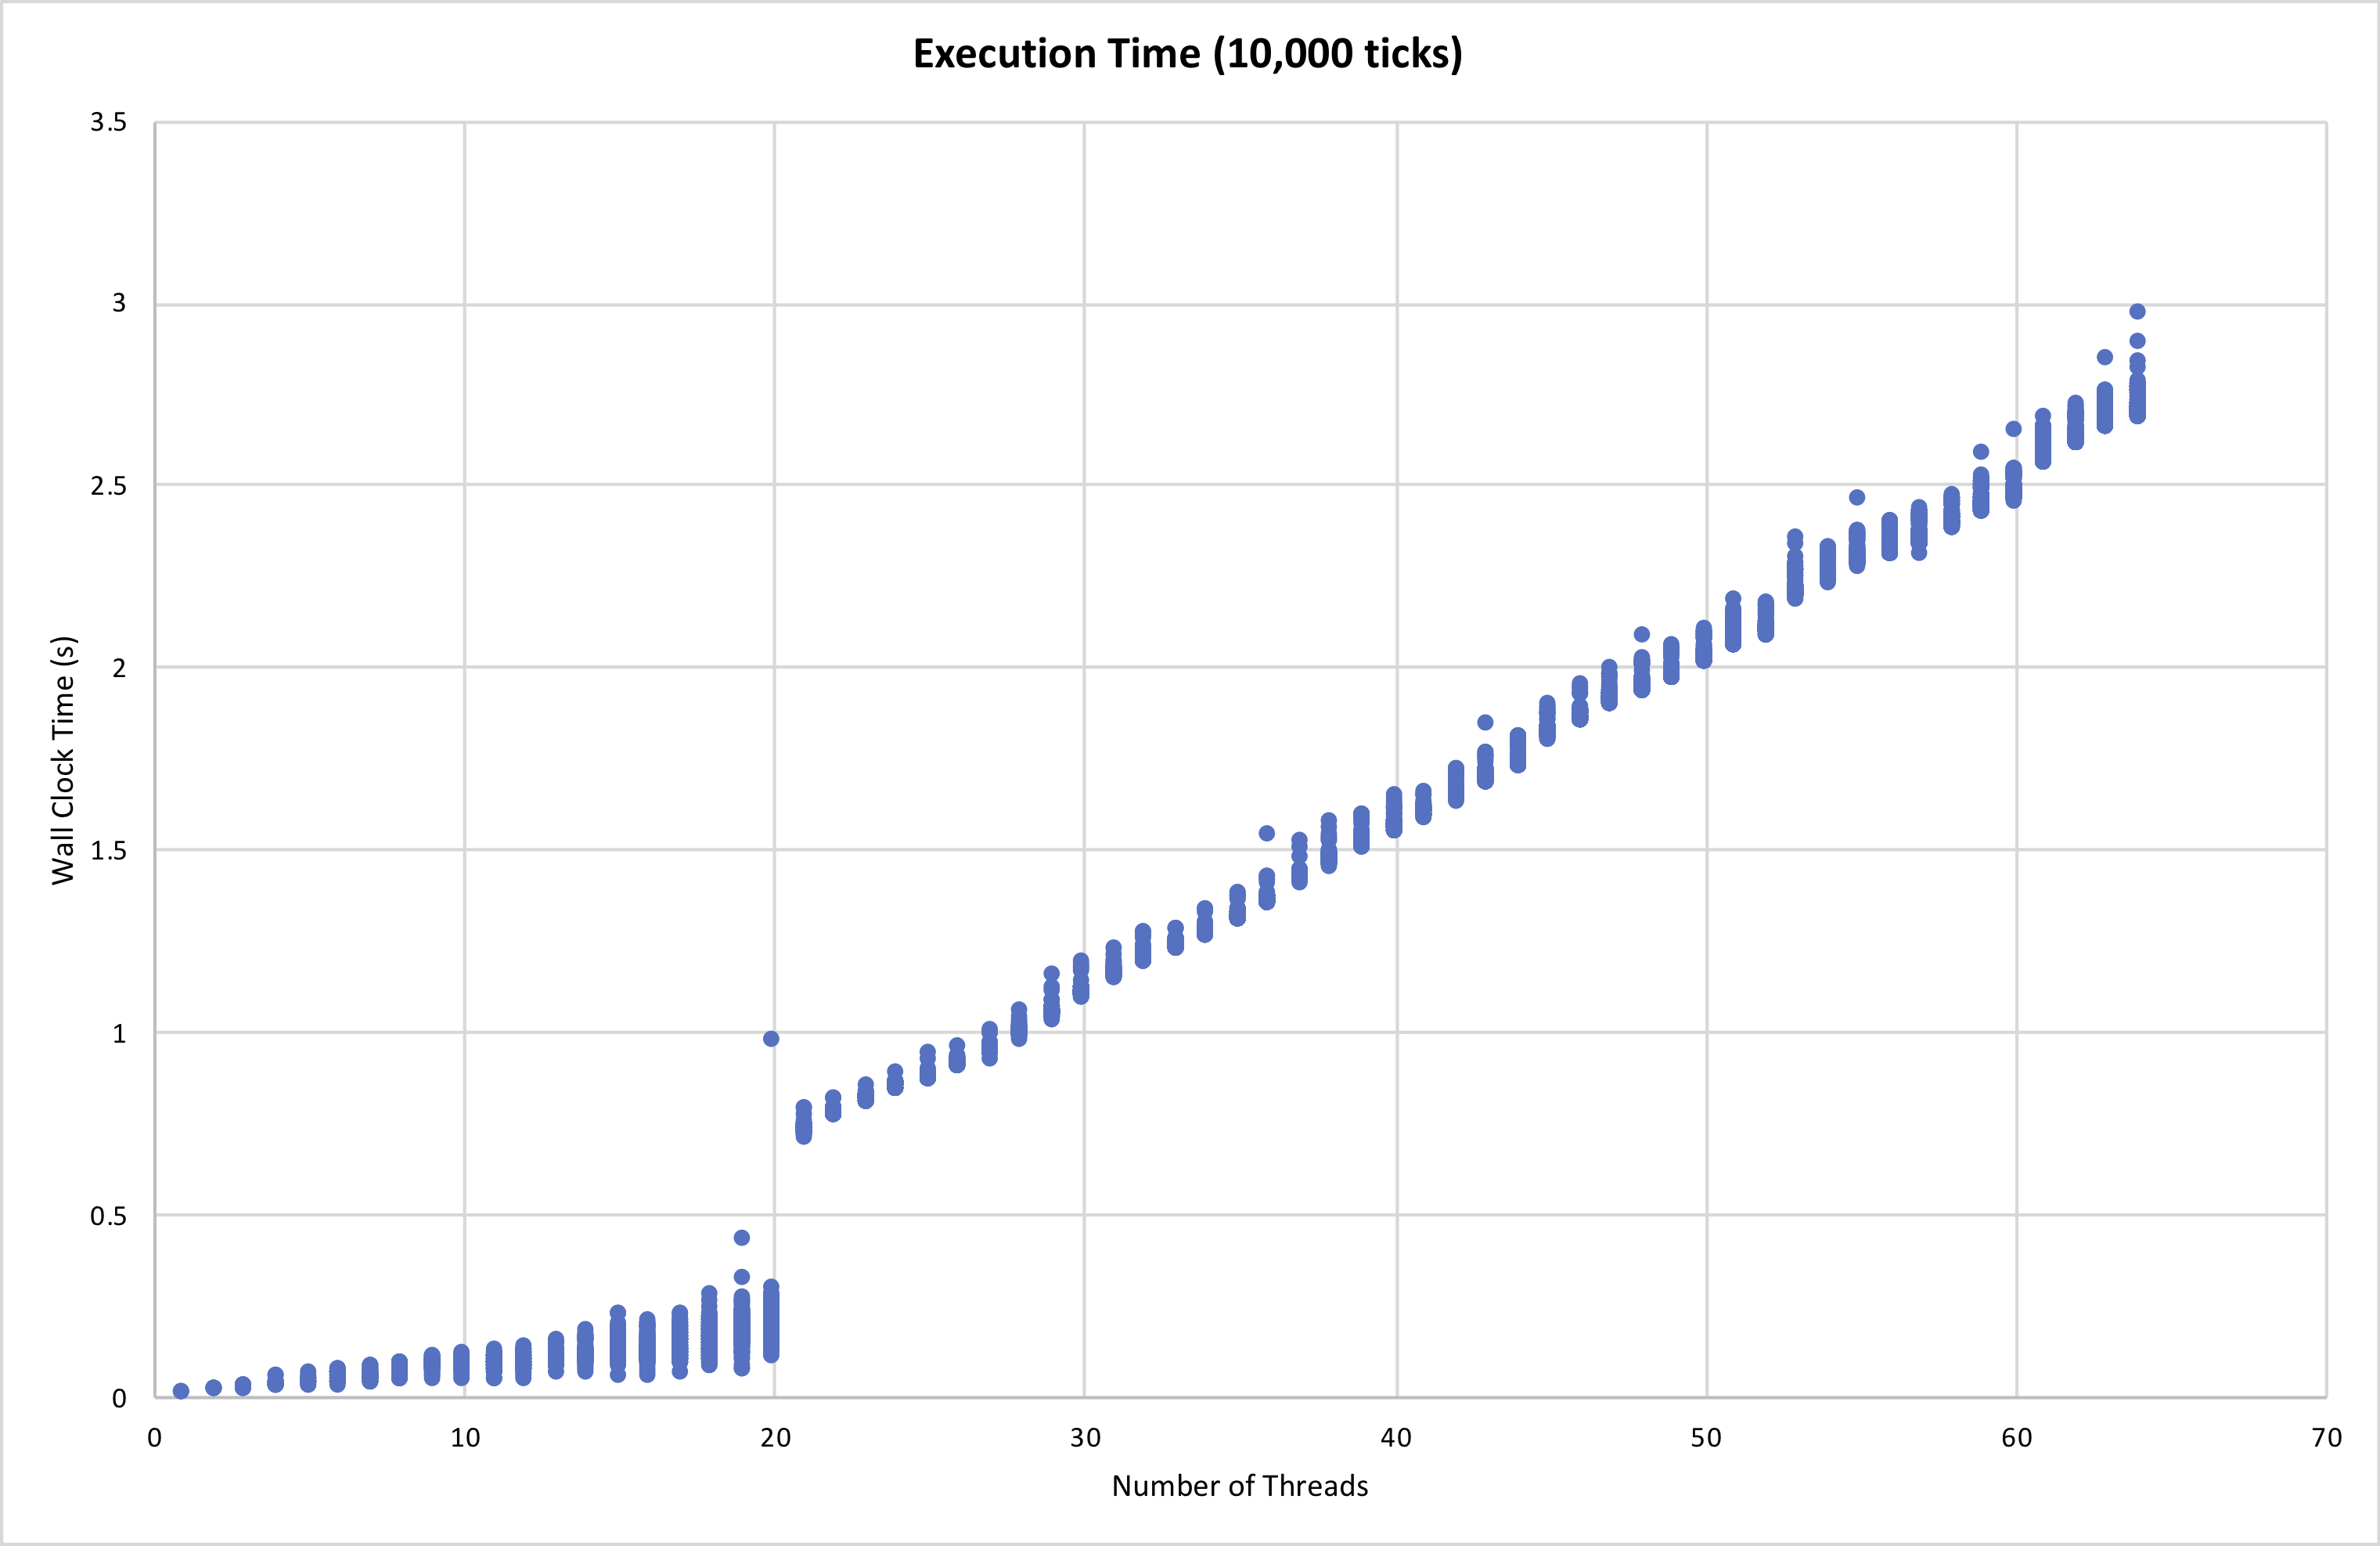
\includegraphics[width=\linewidth]{10000-time}
	\end{center}
	
	\section{Discussion}
	It can be observed that the wall clock time taken for the simulation to complete increases as number of threads increases. This is because as number of threads increases, there is more contention of resources -- in our case contention for each train (thread) in using links (edges) between stations (vertices) and contention for each train in opening door at each station. We are managing this using an implicit queue through implementing a timekeeper to track the next allowed event to occur, protected by a mutex lock. As such, for each link (edge) or station (vertex), only one train (thread) is able to register itself to the timekeeper at any given time -- others will have to wait.
	
	However, we have an interesting observation as well. Notice that the execution time behaves very differently when the number of threads is beyond the number of logical cores (20 cores). For small input size (100 ticks), when the number of threads is beyond the number of logical cores, the execution time actually falls. However, as input size gets larger (1,000 and 10,000 ticks), execution time increases. This can be explained that when the number of threads are below the number of logical cores, all the threads are running concurrently, resulting in more contention. However, when number of threads is above the number of logical cores, the threads take turns to wake up and do work, resulting in less contention. For smaller input size, the contention time actually outweighs the execution time, resulting in the fall in execution time. However, for larger input size, there is a large overhead in context-switching which outweighs the effect of contention time. This is supported by the data we collected on number of context-switches for 100 ticks and 1,000 ticks.
	
	We also observe another trend -- that the variance in execution time falls when the number of threads exceed the number of logical cores. We currently have no explanation on this, but we suspect that the compiler does an optimisation when the number of threads exceed the number of logical cores.
	
	\newpage
	\begin{center}
		\captionof{figure}{Number of context switches for 100 ticks}
		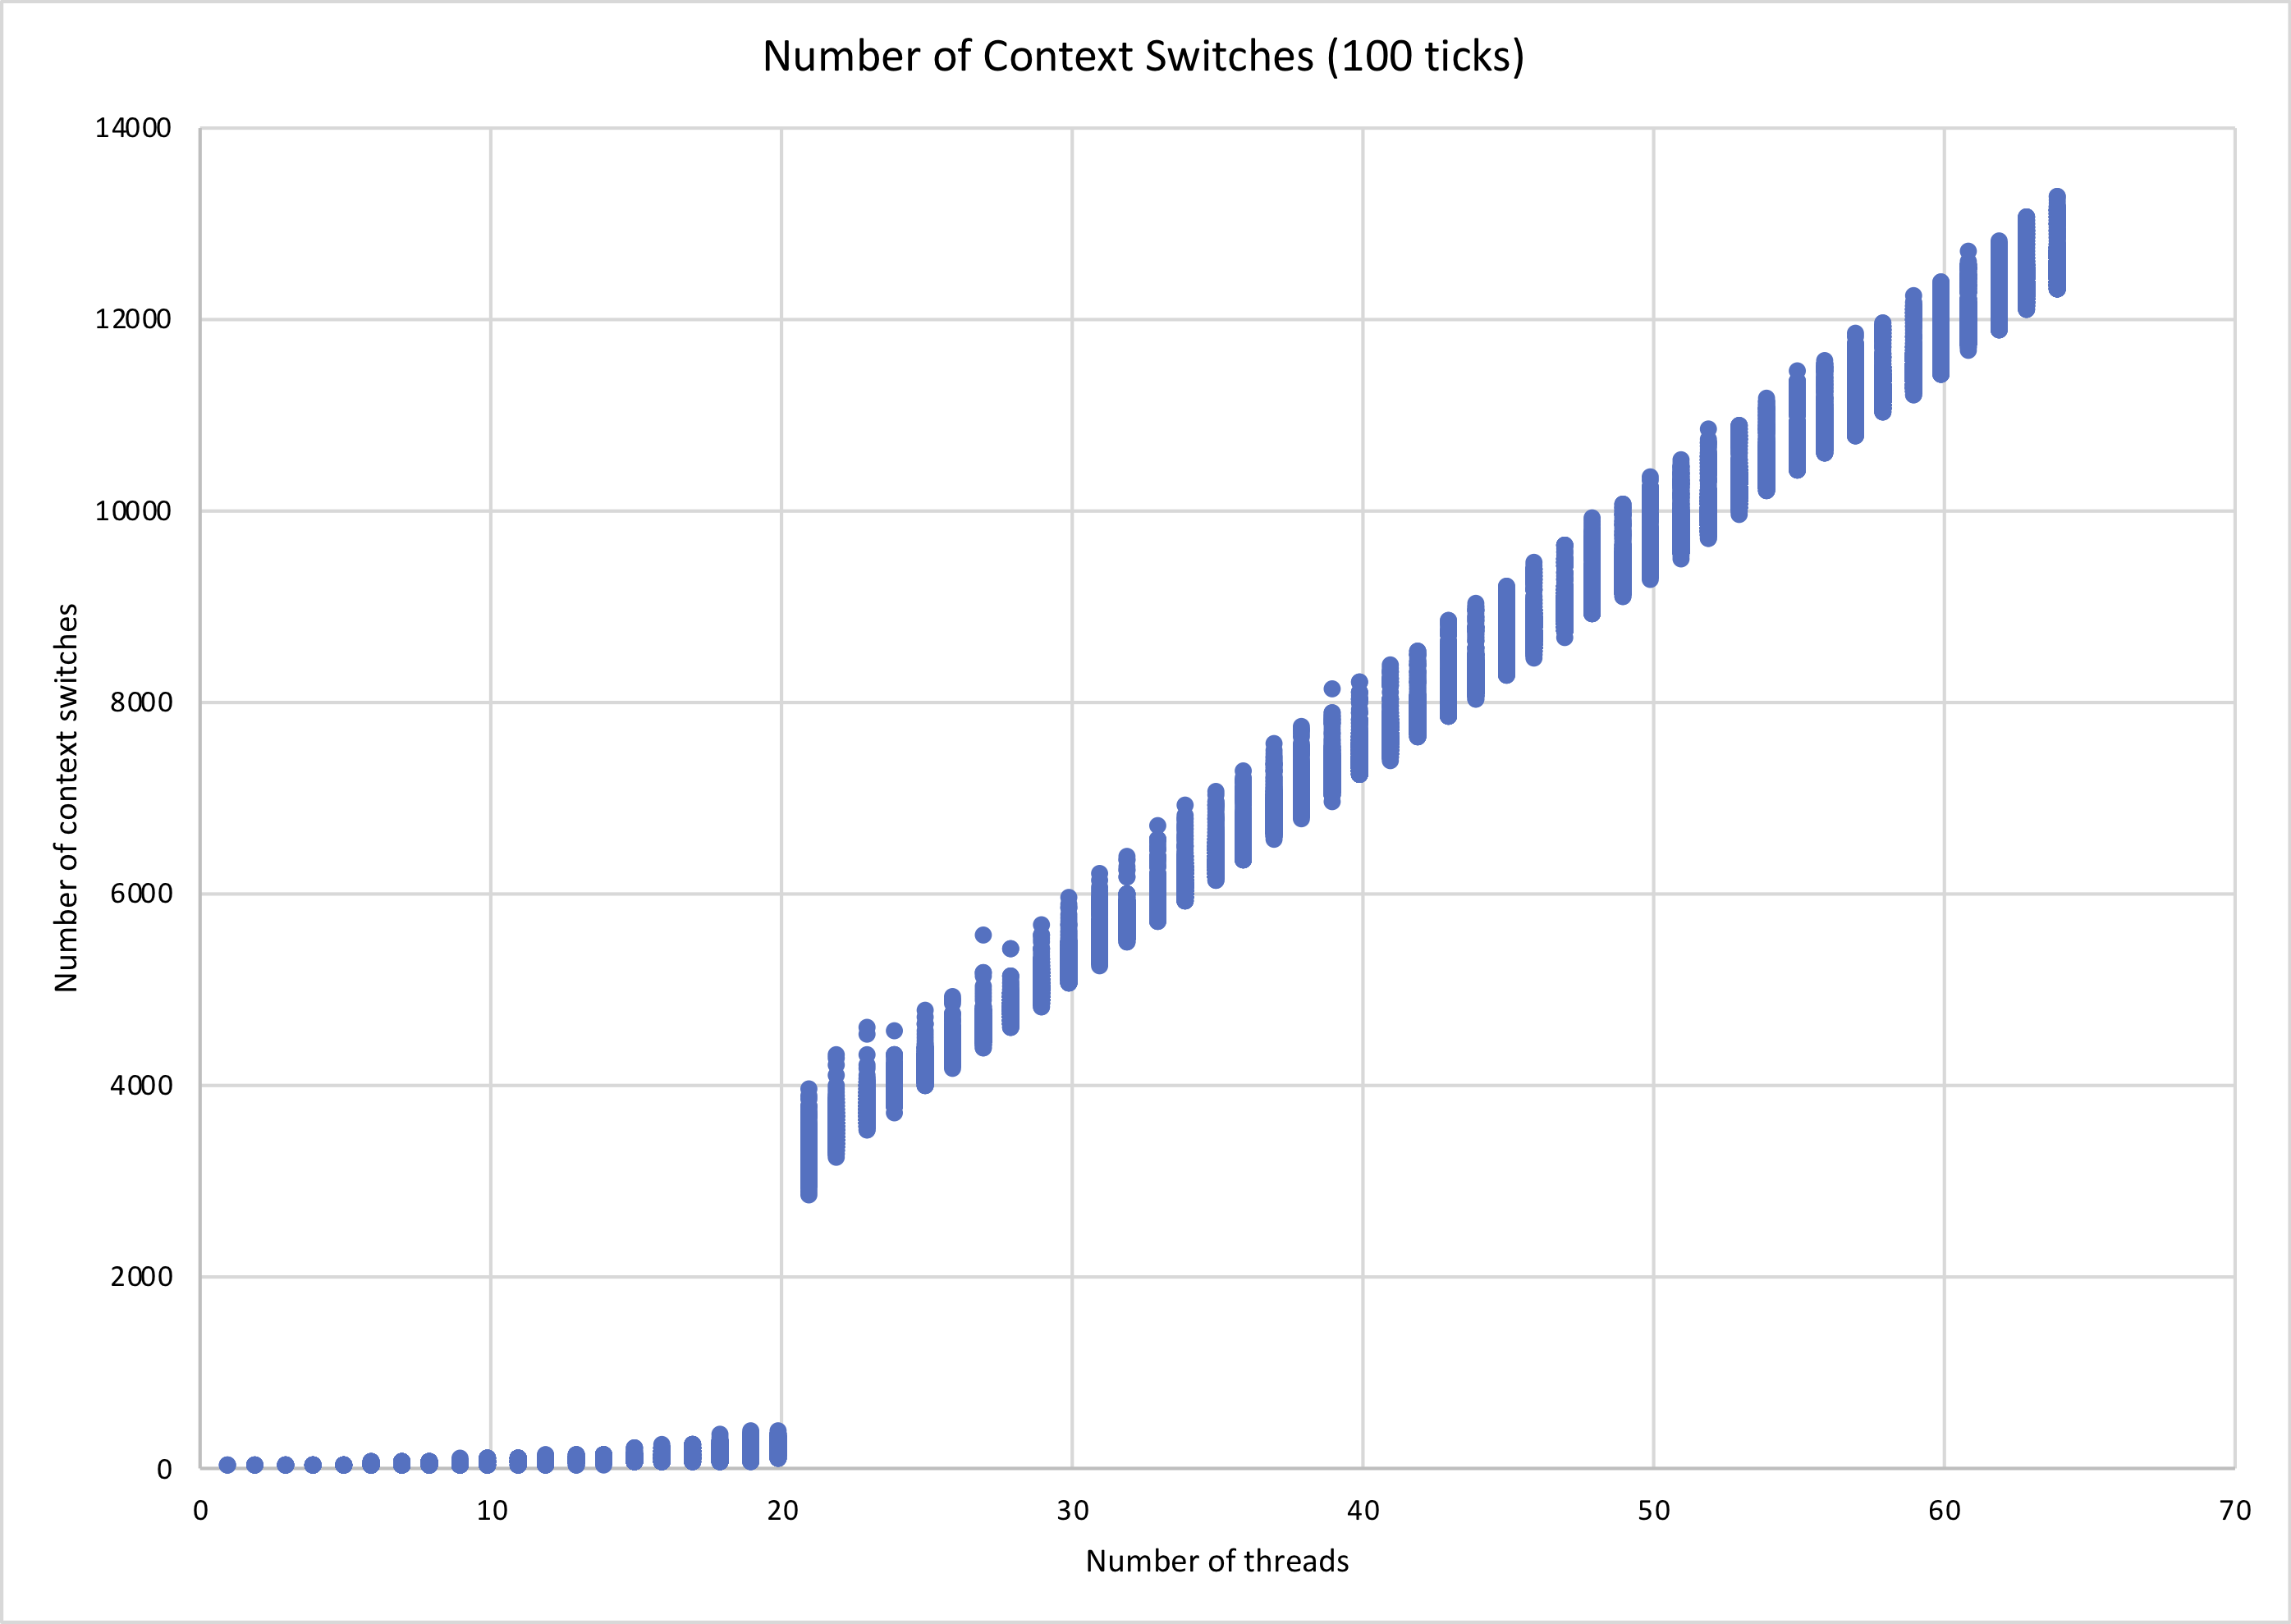
\includegraphics[width=0.9\linewidth]{100-cs}
	\end{center}
	\begin{center}
		\captionof{figure}{Number of context switches for 1,000 ticks}
		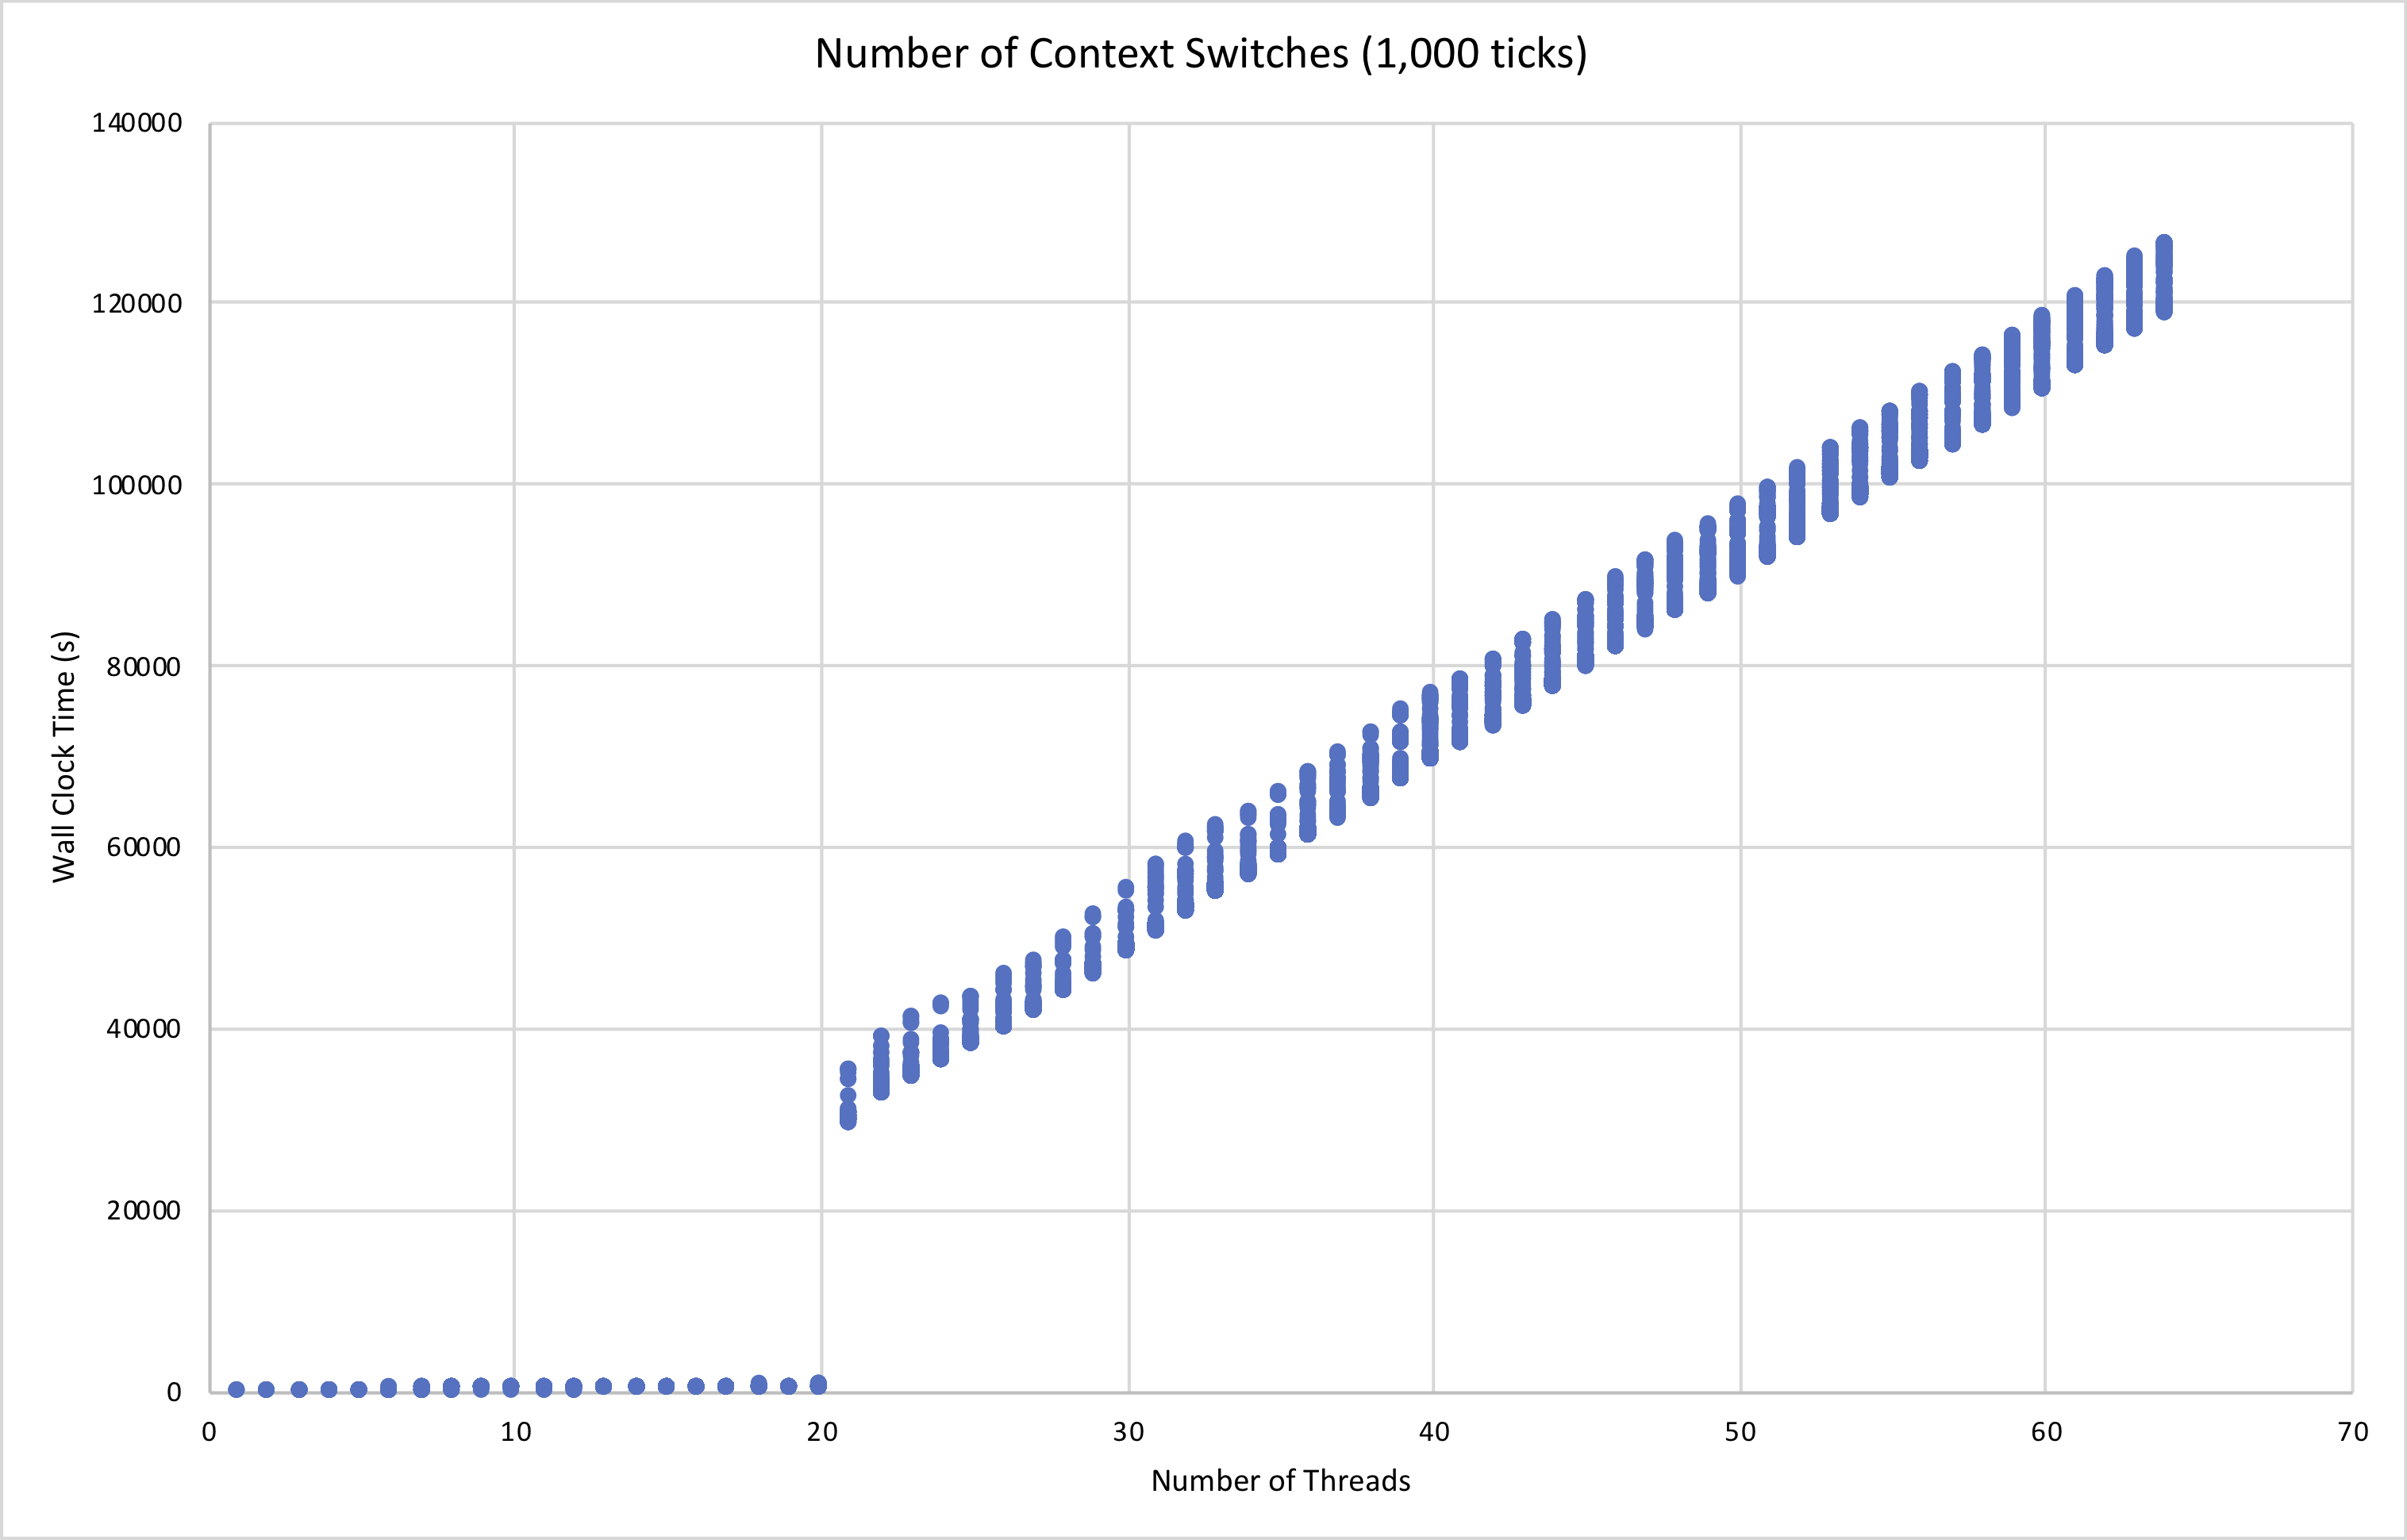
\includegraphics[width=0.9\linewidth]{1000-cs}
	\end{center}
	
	\section{Bonus}
	Starvation will never occur in the simulation program that we wrote. This is because to decide which train to open door or to be allowed to use a link next, we are using an implicit queue to implement First-Come-First-Serve (FCFS) scheduler. As such, every train is assured access to the link or permission to open door aftera long enough time. The assumptions are that no train open its doors or travel using the links indefinitely (which we believe are fair to make).

	\newpage
	\section{Appendix A: Ruby script used to generate test cases}
	Below is the code listing of the ruby script used to generate test cases. Essentially, it does:
	\begin{enumerate}
		\item Create a random adjacency matrix with diagonal = 0
		\item Find the MST of the random graph created
		\item Ensure that there are enough vertices with degree = 1, else go back to step 1
		\item Enumerate the 2-combinations of the vertices with degree = 1, and pick 3 randomly.
		\item For each of the three 2-combinations, assign them to be the termini of each line.
		\item Using breadth-first-search, find the path between the two vertices for each pair of termini.
		\item Ensure that the path is long enough, else go back to step 4.
	\end{enumerate}
	\begin{minted}{Ruby}
require 'set'

MIN_NUM_TERMINI = 4
MIN_NUM_STATIONS_LINE = 4
MRT_STATION_NAMES = ["Jurong East", "Bukit Batok", "Bukit Gombak", "Choa Chu Kang", "Yew Tee", "Kranji", "Marsiling", "Woodlands", "Admiralty", "Sembawang", "Yishun", "Khatib", "Yio Chu Kang", "Ang Mo Kio", "Bishan", "Braddell", "Toa Payoh", "Novena", "Newton", "Orchard", "Somerset", "Dhoby Ghaut", "City Hall", "Raffles Place", "Marina Bay", "Marina South Pier", "Pasir Ris", "Tampines", "Simei", "Tanah Merah", "Bedok", "Kembangan", "Eunos", "Paya Lebar", "Aljunied", "Kallang", "Lavender", "Bugis", "City Hall", "Raffles Place", "Tanjong Pagar", "Outram Park", "Tiong Bahru", "Redhill", "Queenstown", "Commonwealth", "Buona Vista", "Dover", "Clementi", "Jurong East", "Chinese Garden", "Lakeside", "Boon Lay", "Pioneer", "Joo Koon", "Gul Circle", "Tuas Crescent", "Tuas West Road", "Tuas Link", "Expo", "Changi Airport", "HarbourFront", "Outram Park", "Chinatown", "Clarke Quay", "Dhoby Ghaut", "Little India", "Farrer Park", "Boon Keng", "Potong Pasir", "Woodleigh", "Serangoon", "Kovan", "Hougang", "Buangkok", "Sengkang", "Punggol", "Dhoby Ghaut", "Bras Basah", "Esplanade", "Promenade", "Nicoll Highway", "Stadium", "Mountbatten", "Dakota", "Paya Lebar", "MacPherson", "Tai Seng", "Bartley", "Serangoon", "Lorong Chuan", "Bishan", "Marymount", "Caldecott", "Botanic Gardens", "Farrer Road", "Holland Village", "Buona Vista", "one-north", "Kent Ridge", "Haw Par Villa", "Pasir Panjang", "Labrador Park", "Telok Blangah", "HarbourFront", "Bayfront", "Marina Bay", "Bukit Panjang", "Cashew", "Hillview", "Beauty World", "King Albert Park", "Sixth Avenue", "Tan Kah Kee", "Botanic Gardens", "Stevens", "Newton", "Little India", "Rochor", "Bugis", "Promenade", "Bayfront", "Downtown", "Telok Ayer", "Chinatown", "Fort Canning", "Bencoolen", "Jalan Besar", "Bendemeer", "Geylang Bahru", "Mattar", "MacPherson", "Ubi", "Kaki Bukit", "Bedok North", "Bedok Reservoir", "Tampines West", "Tampines", "Tampines East", "Upper Changi", "Expo", "Choa Chu Kang", "South View", "Keat Hong", "Teck Whye", "Phoenix", "Bukit Panjang", "Petir", "Pending", "Bangkit", "Fajar", "Segar", "Jelapang", "Senja", "Ten Mile Junction", "Sengkang", "Compassvale", "Rumbia", "Bakau", "Kangkar", "Ranggung", "Cheng Lim", "Farmway", "Kupang", "Thanggam", "Fernvale", "Layar", "Tongkang", "Renjong", "Punggol", "Cove", "Meridian", "Coral Edge", "Riviera", "Kadaloor", "Oasis", "Damai", "Sam Kee", "Teck Lee", "Punggol Point", "Samudera", "Nibong", "Sumang", "Soo Teck"]

def generate_random_graph(s, max_weight)
  Array.new(s) { |i| Array.new(s) { |j| i == j ? 0 : rand(1..max_weight) } }
end

def print_graph(matrix)
  matrix.map { |row| row.join(' ') }.join("\n")
end

def prim(matrix)
  cost = Array.new(matrix.length, Float::INFINITY)
  parent = Array.new(matrix.length, nil)
  visited = Array.new(matrix.length, false)

  # start from the first vertex
  cost[0] = 0
  parent[0] = -1

  matrix.length.times do
    u = nil
    min_weight = Float::INFINITY

    # Find unvisited vertex with minimum cost
    cost.zip(visited).each_with_index do |zipped, i|
      c, v = zipped
      if c < min_weight and !v
        min_weight = c
        u = i
      end
    end
    visited[u] = true

    matrix[u].zip(cost, visited).each_with_index do |zipped, i|
      m, c, v = zipped
      if m > 0 && !v && c > m
        cost[i] = m
        parent[i] = u
      end
    end
  end

  result = Array.new(matrix.length) { Array.new(matrix.length, 0) }

  (1...matrix.length).each do |i|
    result[i][parent[i]] = result[parent[i]][i] = matrix[i][parent[i]]
  end

  result
end

def bfs(matrix, termini)
  from, to = termini
  open_set = []
  closed_set = Set[]
  meta = {}

  root = from
  meta[root] = nil
  open_set.unshift(root)

  while !open_set.empty? do
    subtree_root = open_set.shift
    if subtree_root == to
      return construct_path(subtree_root, meta)
    end
    matrix[subtree_root].each_with_index.select { |w, i| w > 0 }.map { |x| x.last }.each do |child|
      next if closed_set.include?(child)
      if !open_set.include?(child)
        meta[child] = subtree_root
        open_set.unshift(child)
      end
    end
    closed_set.add(subtree_root)
  end
end

def construct_path(state, meta)
  result = [state]
  while !meta[state].nil? do
    state = meta[state]
    result.append(state)
  end
  result.reverse
end

def permutate_sum(n)
  (0..n).to_a.flat_map { |i| (0..(n - i)).to_a.map { |j| [i, j, n - i - j] } }
end

def usage_message
  puts "Invalid args"
  puts "Usage: ruby test_case_generator.rb <num_vertex> <max_weight> <num_tick>"
  exit 1
end

# Start of main
if ARGV.length != 3
  usage_message
end

s, max_weight, tick = ARGV.map { |a| a.to_i }

if s <= 0 || max_weight <= 0
  usage_message
end

primmed = nil
termini = []

while termini.length < MIN_NUM_TERMINI do
  graph = generate_random_graph(s, max_weight)
  primmed = prim(graph)
  termini = primmed
    .each_with_index.select do |row, i|
      row.reduce(0) { |acc, weight| acc += weight > 0 ? 1 : 0 } == 1
    end
    .map { |pair| pair.last }
end

stations = MRT_STATION_NAMES.sample(s)
popularities = Array.new(s) { rand(1..10) / 10.0 }

green_line = []
yellow_line = []
blue_line = []
while green_line.length < MIN_NUM_STATIONS_LINE || yellow_line.length < MIN_NUM_STATIONS_LINE || blue_line.length < MIN_NUM_STATIONS_LINE do
  green_termini, yellow_termini, blue_termini = termini.combination(2).to_a.sample(3)

  green_line = bfs(primmed, green_termini)
  yellow_line = bfs(primmed, yellow_termini)
  blue_line = bfs(primmed, blue_termini)
end

dir_name = "test-#{Time.now.strftime("%Y%m%d-%H%M")}"
Dir.mkdir(dir_name)

(1..64).each do |n|
  puts "Generating test cases for #{n} threads"
  permutate_sum(n).each do |trains|
    File.open("#{dir_name}/#{trains.join("-")}", "w") do |f|
      f.puts s
      f.puts stations.join(",")
      f.puts print_graph(primmed)
      f.puts popularities.join(",")
      f.puts green_line.map { |s| stations[s] }.join(",")
      f.puts yellow_line.map { |s| stations[s] }.join(",")
      f.puts blue_line.map { |s| stations[s] }.join(",")
      f.puts tick
      f.puts trains.join(",")
    end
  end
end

	\end{minted}
\end{document}